\documentclass[a4paper,10pt]{report}

\usepackage{listings}
\usepackage{color}

\renewcommand\lstlistingname{Quelltext} % Change language of section name

\lstset{ % General setup for the package
	language=C,
	basicstyle=\small\sffamily,
	numbers=left,
 	numberstyle=\tiny,
	frame=tb,
	tabsize=4,
	columns=fixed,
	showstringspaces=false,
	showtabs=false,
	keepspaces,
	commentstyle=\color{red},
	keywordstyle=\color{blue}
}
\renewcommand{\thesection}{}
\usepackage[utf8]{inputenc}
\usepackage[tc]{titlepic}
\usepackage{xcolor}
\usepackage{graphicx}
\usepackage{amsmath}
\usepackage{geometry}
\usepackage{tikz}
\usetikzlibrary{shapes.geometric, arrows}
\geometry{
 a4paper,
 total={170mm,257mm},
 left=20mm,
 top=20mm,
 }

\definecolor{title}{RGB}{180,0,0}
\definecolor{other}{RGB}{171,0,255}
\definecolor{name}{RGB}{255,0,0}
\definecolor{phd}{RGB}{0,0,240}

\title{\textbf{Assignment-6\\
ELP - 718 Telecom Software Laboratory}}

\author{Shefali Gupta}

\date{\parbox{\linewidth}{\centering%
  \today\endgraf\bigskip
 Entry No. - 2017JTM2767\endgraf\bigskip
  \includegraphics[width=2cm]{/home/shefaligupta/Downloads/iit.png} \endgraf\bigskip
Bharti School\\
Telecommunication Technology and Management \\ IIT DELHI\\India}}

\begin{document}

\pagenumbering{gobble}
\maketitle

\newpage
\tableofcontents
\newpage
\pagenumbering{arabic}

\section{Problem Statement}

\paragraph{Parity Check}
Take the input bit stream and append a single bit, called a parity check. This parity check bit has the value 1 if number of 1’s in the bit string is even and has the value 0 otherwise, i.e., Odd Parity Check.

\paragraph{Bit Oriented Framing}

Data Link Layer needs to pack bits into frames, so that each frame is distinguishable from another. Frames can be fixed or variable size. In variable size framing, we define end of frame using bit oriented approach. It uses a special string of bits, called a flag for both idle fill and to indicate the beginning and the ending of frames.
The string 0101 is used as the bit string or flag to indicate the end of the frame. The bit stuffing rule is to insert a 0 after each appearance of 010 in the original data. In addition, if the frame ends in 01, a 0 would be stuffed after the 1st 0 in the actual terminating string 0101

%\subsection{Assumptions}

\subsection{Program Structure}


% Define block styles
\tikzstyle{decision} = [diamond, draw, fill=blue!20, 
    text width=4em, text badly centered, node distance=3cm, inner sep=0pt]
\tikzstyle{block} = [rectangle, draw, fill=blue!20, 
    text width=9em, text centered, rounded corners, minimum height=4em]
\tikzstyle{line} = [draw, -latex']
\tikzstyle{cloud} = [draw, ellipse,fill=red!20, node distance=3cm,
    minimum height=2em]
\begin{center}
 

  
\begin{tikzpicture}[node distance = 2cm, auto]
      % Place nodes
    \node [cloud] (init) {start};
    \node [block, below of=init] (identify) {Take the bit data stream from user};
    \node [decision, below of=identify, node distance=2.5cm] (evaluate) {count the total no of one's};
    \node [block, left of=evaluate, node distance=5cm] (update) {if number of one's is even then add '1' at the end of bit data};
    \node [block, right of=update, node distance=10cm] (result1) {if number of one's is odd then add '0' at the end of bit data };
    \node [decision, below of=evaluate, node distance=4cm] (result2) {check the bit pattern '010' in original message};
    \node [block, left of=result2, node distance=5cm] (again) {if pattern found then add '0' after the pattern};
    \node [block, right of=result2, node distance=5cm] (again1) {if pattern not found then do nothing};
    \node [block, below of=result2, node distance=3	cm] (result3) {Add the flag stream '0101' to indicate the ending of frames};
    \node [block, below of=result3, node distance=2.5	cm] (result4) {print the final modified data bit stream};
    \node [cloud, below of=result4, node distance=2cm] (stop) {stop};
    % Draw edges
    \path [line] (init) -- (identify);
    \path [line] (identify) -- (evaluate);
    \path [line] (evaluate) --(update);
    \path [line] (evaluate) --(result1);
    \path [line] (evaluate) --(result2);
  %  \path [line] (update) -- (result1);
   % \path [line] (result1) -- (result2);
    \path [line] (result2) -- (again);
    \path [line] (result2) -- (again1);
  %  \path [line] (again) |- (result1);
    \path [line] (result2) -- (result3);
    \path [line] (result3) -- (result4);
    \path [line] (result4) -- (stop);
\end{tikzpicture}

\end{center}


\subsection{Algorithm and Implementation}

\begin{itemize}
 \item Take the input of data bits from user.
 \item Check the odd parity and add the parity bit at the end of bit stream.
 \item Check the bit pattern '010' in the updated message bits, if pattern found then add the '0' at the end of pattern.
 \item Check the last two bits of updated data bits, if frame ends in '01' then a '0' would be added after the 1st 0 in the actual terminating string 0101.
 \item At the end of frame add the flag '0101' to indicate the end of frame.
\end{itemize}

%\subsection{Source Code}

%\lstinputlisting{client.c}

\subsection{Input and Output Format}

\paragraph{Input}

Take the input - 01010

\paragraph{Output}

First output after adding parity bit - 010101\\
Second output after bit stuffing - 0100100100101


\subsection{Test Cases}

\begin{itemize}
 \item Take the input data bit from user - 01010
 \item Check the odd parity. Number of 1's is even then output should be - 010101
 \item check the pattern '010'. output should be - 0100100100101
\end{itemize}


%\subsection{Difficulties/Issues Faced}

\subsection{Screenshots}
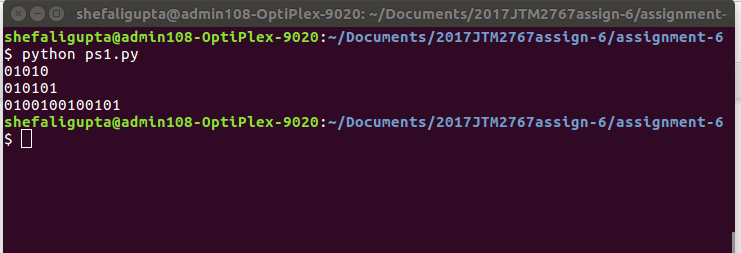
\includegraphics[width=10cm]{/home/shefaligupta/Documents/2017JTM2767assign-6/ps1.png}

\section{Problem Statement-2}

3X3 Numeric Tic-Tac-Toe (Use numbers 1 to 9 instead of X’s and O’s)
One player plays with the odd numbers (1, 3, 5, 7, 9) and other player plays with the even numbers (2,4,6,8). All numbers can be used only once. The player who puts down 15 points in a line wins (sum of 3 numbers). Always Player with odd numbers start the game. Once a line contains two numbers whose sum is 15 or greater, there is no way to complete that line, although filling in the remaining cell might be necessary to complete a different line.
Note – Line can be horizontal, vertical or diagonal


\subsection{Assumptions}
Assume that player 1 has all odd numbers and player 2 has all even numbers.

\subsection{Program Structure}

% Define block styles
\tikzstyle{decision} = [diamond, draw, fill=blue!20, 
    text width=4em, text badly centered, node distance=3cm, inner sep=0pt]
\tikzstyle{block} = [rectangle, draw, fill=blue!20, 
    text width=9em, text centered, rounded corners, minimum height=4em]
\tikzstyle{line} = [draw, -latex']
\tikzstyle{cloud} = [draw, ellipse,fill=red!20, node distance=3cm,
    minimum height=2em]
\begin{center}
 

  
\begin{tikzpicture}[node distance = 2cm, auto]
      % Place nodes
    \node [cloud] (init) {start};
    \node [block, below of=init] (identify) {start the game with player 1};
    \node [block, below of=identify, node distance=2.5cm] (evaluate) {take the position and value as a input from player };
    \node [block, below of=evaluate, node distance=2.5cm] (update) {put the value at given position in matrix};
    \node [block, below of=update, node distance=3cm] (result1) {Give the chance to next player };
    \node [decision, below of=result1, node distance=5cm] (result2) {check the sum of all horizontal blocks,vertical blocks and digonl bolck};
    \node [block, left of=result2, node distance=5cm] (again) {If sum is less than 15};
    \node [block, below of=result2, node distance=4	cm] (result3) {If sum is equal or greater than 15};
    \node [block, below of=result3, node distance=2.5	cm] (result4) {Terminate the game and show the winner};
    \node [block, below of=result4, node distance=2.5	cm] (result5) {Ask the players for the next game};
    \node [cloud, below of=result5, node distance=2cm] (stop) {stop};
    % Draw edges
    \path [line] (init) -- (identify);
    \path [line] (identify) -- (evaluate);
    \path [line] (evaluate) -- (update);
    \path [line] (update) -- (result1);
    \path [line] (result1) -- (result2);
    \path [line] (result2) -| node [near start] {No} (again);
    \path [line] (again) |- (result1);
    \path [line] (result2) -- node {yes}(result3);
    \path [line] (result3) -- (result4);
    \path [line] (result4) -- (result5);
    \path [line] (result5) -- (stop);
\end{tikzpicture}

\end{center}

\subsection{Algorithm and Implementation}

\begin{itemize}
 \item Start the game with '0' at all position in matrix.
 \item Take the input of position and value from player.
 \item Put the value in matrix at given position.
 \item Give the chance to next player.
 \item And do same as defined in step 2 and 3.
 \item Calculate the sum of all horizontal blocks,vertical blocks and digonl bolck.
 \item If sum is less than 15 then continue the game.
 \item If sum is equal or greater than 15 then terminate the game and display the winner.
 \item Ask for next game to the players, if they want to play then repeat all above steps.

\end{itemize}

%\subsection{Source Code}

%\lstinputlisting{client.c}

\subsection{Input and Output Format}

\paragraph{Input}

Take the input - position,value\\
Enter the position and number to be entered from user\\
Ex. - 5,3


\paragraph{Output}
Output will look like this:\\

\begin{center}
 0 0 0\\
 0 3 0\\
 0 0 0\\

\end{center}




\subsection{Test Cases}

\begin{itemize}
 \item Take the position and number as input from user.
 \item Insert the number at given position in matrix.
 \item if sum of any horizontal block, vertical block and digonal block is greater than or equal 15 then game should be terminate.
 \item if sum is less than 15 then next player chance should come.
 
\end{itemize}


%\subsection{Difficulties/Issues Faced}

\subsection{Screenshots}
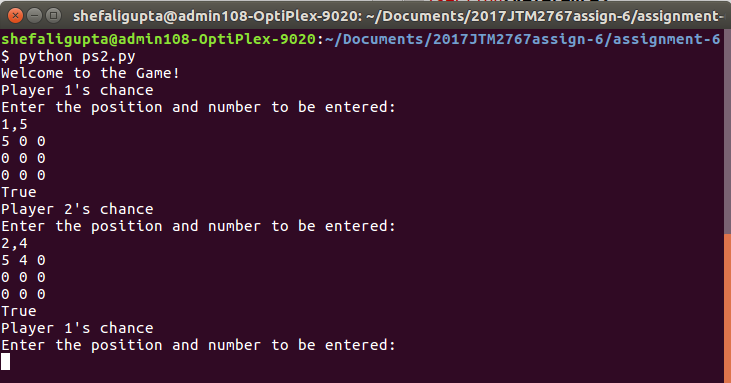
\includegraphics[width=10cm]{/home/shefaligupta/Documents/2017JTM2767assign-6/ps2.png}


\section{Reference}

\begin{thebibliography}{9}
 \bibitem{C Basic tutorial}
 C Basic tutorial\\
 \textit{http://www.cprogramming.com/tutorial/c-tutorial.html\\ http://www.tutorialspoint.com/cprogramming/ \\ http://www.ime.usp.br/~pf/Kernighan-Ritchie/C-Programming-Ebook.pdf}
 
 \bibitem{Video tutorials}
 Vedio tutorial\\
 \textit{https://www.youtube.com/watch?v=Yq6XFl-u00o}\\
 \textit{https://www.youtube.com/watch?v=sCtY--xRUyI}\\
 \textit{https://www.youtube.com/watch?v=xQ0ONbt-qPs}\\
 
 \bibitem{GDB}
 GDB \\
 \textit{https://www.cs.umd.edu/~srhuang/teaching/cmsc212/gdb-tutorial-handout.pdf}
\end{thebibliography}

\section{Source code}

\subsection{Source Code -1}

\lstinputlisting{ps1.py}

\subsection{Source Code - 2}

\lstinputlisting{ps2.py}



\end{document}          
